\section{Penyajian Data Uji Coba}

Pada penelitian ini dilakukan uji coba menggunakan data lokasi seluruh SMA di Kabupaten Probolinggo, dan dijalankan menggunakan python. Berikut adalah sajian data hasil uji coba.

\subsection{Pengambilan Data Lokasi}

Data yang digunakan adalah data koordinat lokasi yang diekspor memalui google earth. Pengujian Pengambilan data lokasi bertujuan untuk menunjukkan bahwa sistem 
mampu membaca input yang dimasukkan. Dapat dilihat pada Gambar \ref{fig:datalok} sebagian nama nama sekolah di kabupaten probolinggo beserta koordinat lokasinya. Visualisasi data dari koordinat-koordinat SMA di kabupaten probolinggo dapat dilihat pada Gambar \ref{fig:petasma}.

\begin{figure}[h!]
  \centering
  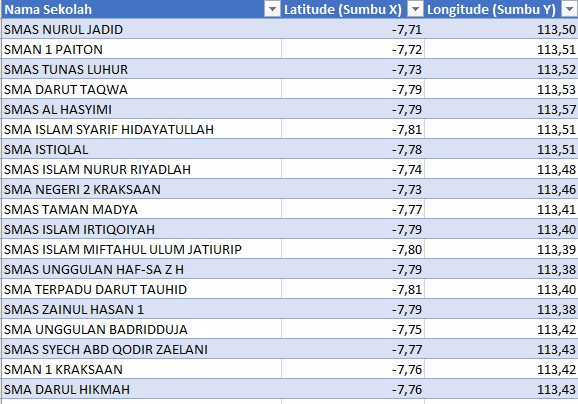
\includegraphics[width=0.8\textwidth]{data lokasi sekolah.png}
  \caption{Beberapa Data Lokasi Sekolah}
  \label{fig:datalok}
\end{figure}

\begin{figure}[h!]
  \centering
  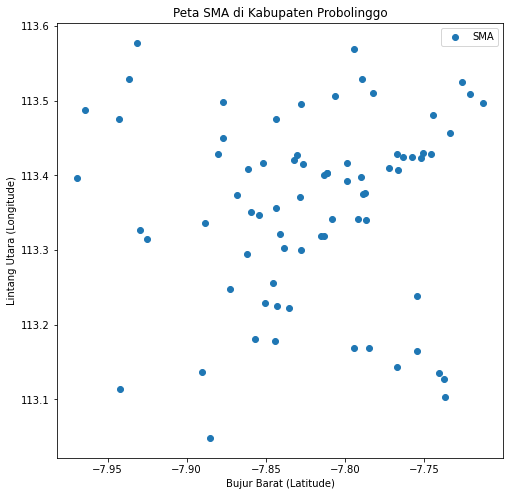
\includegraphics[width=0.8\textwidth]{peta sma.png}
  \caption{Visualisasi lokasi SMA di Kabupaten Probolinggo}
  \label{fig:petasma}
\end{figure}

Setelah mendapatkan lokasi yang akan diproses, selanjutnya adalah menentukan beberapa titik centroid secara random, dalam penelitian ini akan diambil 10 centroid secara random seperti pada Gambar \ref{fig:dasen} dan \ref{fig:visdasen}.

\begin{figure}[h!]
	\centering
	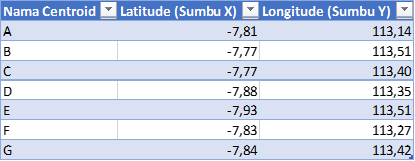
\includegraphics[width=0.8\textwidth]{centroid.png}
	\caption{Data Centroid}
	\label{fig:dasen}
\end{figure}

\begin{figure}[h!]
	\centering
	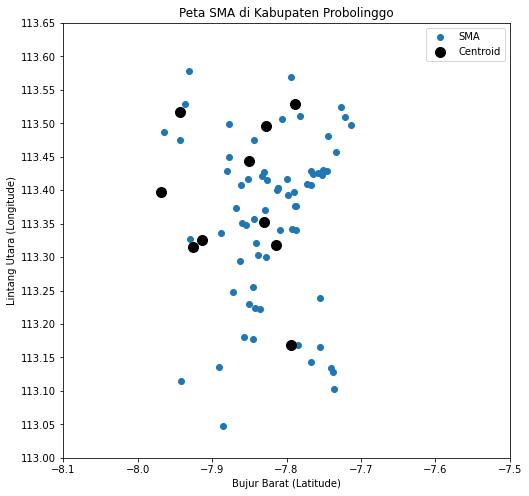
\includegraphics[width=0.8\textwidth]{titik centroid.png}
	\caption{Data Koordinat Centroid}
	\label{fig:visdasen}
\end{figure}

\subsection{Proses Pengklasteran Data}

Pada tahap ini metode yang digunakan adalah metode $K-$means untuk mengklaster data. Langkah-langkah nya adalah sebagai berikut.

\begin{enumerate}
	\item Menentukan jumlah klaster, dalam hal ini ditetapkan adalah 10 klaster.
	\item Menentukan titik centroid secara random seperti pada Gambar \ref{fig:dasen} dan \ref{fig:visdasen}
	\item Pengklasifikasian data, dalam langkah ini akan dikelompokkan data sesuai dengan titik centroid paling dekatnya dengan menggunakan rumus \textit{Euclidean Distance} seperti Persamaan \ref{eq:euclidean3}.
	
	\begin{equation}
	\left[ \left( x,y \right) ,\left( a,b \right)\right]=\sqrt{\left( x-a \right)^{2}+\left( y-b \right)^{2}}
	\label{eq:euclidean3}
	\end{equation}
	
	\item Setelah semua data terklasifikasi, selanjutnya adalah memperbarui titik-titik centroid dengan cara menghitung rata-rata tiap anggota klaster.
\end{enumerate}